\makeheading{Lecture 14 | 2020-10-28}
\underline{Model Selection}
\begin{itemize}
      \item Criteria: $ R^2_{\text{adj}} $, AIC, BIC,
            MSPE, etc.\ explicitly penalizes unnecessarily
            complex models.
      \item Search strategies (use with chosen
            criterion)
\end{itemize}
\begin{enumerate}[label=(\roman*)]
      \item Brute force: fit all possible regressions.
            With $ p $ predictors, we have
            $ \sum_{j=0}^{p} \binom{p}{j}=2^p $ possible models to fit.
            \begin{itemize}
                  \item Finds optimal model that may be computationally
                        intensive (or infeasible) if $ p $ is large.
            \end{itemize}

            \underline{Idea}: Find a ``good'' (useful)
            model in reasonable computational time (not necessarily optimal).
            Many strategies focus on adding/removing variables one at a time.
      \item Forward selection: add one variable at a time to model.
            \begin{itemize}
                  \item Start with a model that only has an intercept $ (\beta_0) $.
                  \item Fit $ p $ simple linear regression models
                        \[ \symbf{y}=\beta_0 \symbf{1}+\beta_1\symbf{x}_j
                              +\symbf{\varepsilon}\quad j=1,\ldots,p \]
                  \item Pick the best of $ p $ models (with 1 predictor)
                        according to chosen criterion, and add that variable
                        $ x_j $ to model.
                  \item Fit $ (p-1) $ models containing $ x_j $
                        and one other variable.
                        \begin{itemize}
                              \item If none of $ (p-1) $ models improves
                                    criterion, stop.
                              \item Pick the best of $ (p-1) $ models according
                                    to criterion, so now we have $ 2 $ variables in the model.
                        \end{itemize}
            \end{itemize}
            Continue adding $ 1 $ variable at a time in this way until
            we can no more variables improve the criterion. The final
            model is one with the best criterion after we \emph{stop};
            that is, no further improvement is possible.

            \underline{Note}: Much faster than brute force as the
            maximum number of models to fit is:
            \[ p+(p-1)+\cdots+2+1=\sum_{i=1}^{p}i=\frac{p(p+1)}{2} \]
            which is $ \mathcal{O}(p^2) $ compared to $ \mathcal{O}(2^p) $
            for all possible regressions.
      \item Backward direction: remove one variable at a time to model.
            \begin{itemize}
                  \item Start with model that has $ p $ predictors.
                  \item Fit $ p $ models that result from removing one variable
                        from the regression; that is, each one has $ (p-1) $
                        variables.
                  \item Pick the best of $ p $ models according to criterion.
                        \begin{itemize}
                              \item Eliminate that variable $ x_j $ from model.
                              \item Fit $ (p-1) $ models that remove $ x_j $
                                    and one other variable from model.
                              \item Pick best of $ (p-1) $ models
                                    (2 variables removed).
                        \end{itemize}
            \end{itemize}
            Continue removing $ 1 $ variable at a time in this way until
            we can no more variables improve the criterion. Same computational
            complexity as forward selection.
      \item Forward-backwards (allows individual variables to be both added/removed)
            \begin{itemize}
                  \item Start as in forward selection
                  \item If we have $ k $ variables in model:
                        \begin{itemize}
                              \item Backwards: fit $ k $ models with $ (k-1) $
                                    variables. If any of these improve criterion,
                                    remove the variable.
                              \item Forwards: fit $ (p-k) $ models with $ (k+1) $
                                    variables. If any of these improve criterion,
                                    add that variable.
                        \end{itemize}
            \end{itemize}
\end{enumerate}
\begin{itemize}
      \item These are the basic ``stepwise'' selection models to get
            a ``good'' (useful) model.
      \item Many other have sophisticated procedures available.
            For example, stochastic search, lasso.
      \item We've assumed that $ n>p $ because otherwise
            $ (X^\top X) $ is not invertible. More specialized
            methods needed if number of predictors is larger than sample size.
\end{itemize}
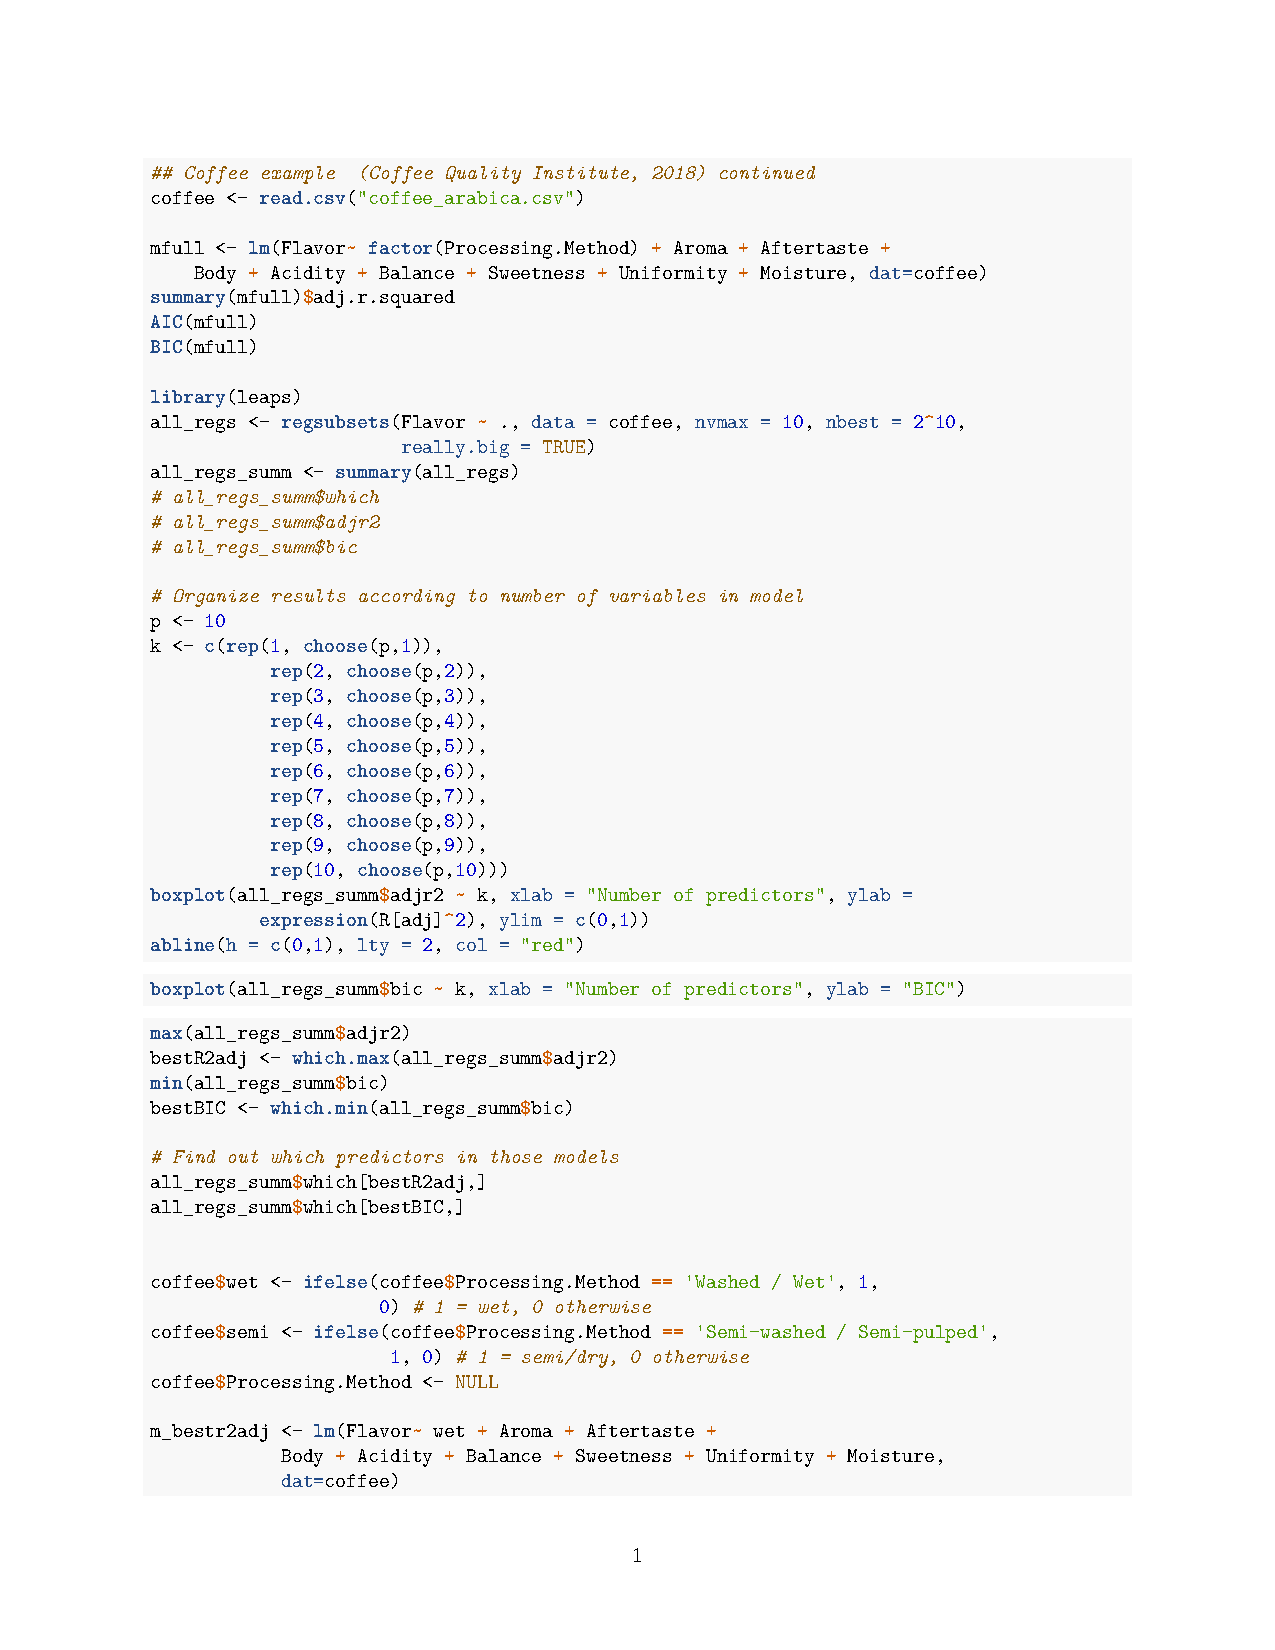
\includepdf[pages=-]{model-selection-basic}
